% TEXINPUTS=.:$HOME/git/bvtex: latexmk  -pdf <main>.tex
\documentclass[xcolor=dvipsnames]{beamer}

\input{defaults}
\input{beamer/preamble}

\setbeamertemplate{navigation symbols}{}
% \setbeamertemplate{background}[grid][step=1cm]

\usepackage{siunitx}
\usepackage{xmpmulti}
\usepackage[export]{adjustbox}
\usepackage{ulem}
\usepackage[outline]{contour}
\usepackage{pdfpages}
\usepackage{tikz}
\usetikzlibrary{shapes.geometric, arrows}
\usetikzlibrary{positioning}

\definecolor{bvtitlecolor}{rgb}{0.98, 0.92, 0.84}
\definecolor{bvoutline}{rgb}{0.1, 0.1, 0.1}

\renewcommand{\bvtitleauthor}{Brett Viren}
\renewcommand{\bvtit}{WCT sim}
\renewcommand{\bvtitle}{\LARGE WCT Simulation Developments\\and larsoft integration}
\renewcommand{\bvevent}{{\small Yale Visit to BNL -- 12 Apr 2018}}
\renewcommand{\bvdate}{12 Apr 2018}
\renewcommand{\bvbeamerbackground}{}

\def\Put(#1,#2)#3{\leavevmode\makebox(0,0){\put(#1,#2){#3}}}

\begin{document}
\input{beamer/title.tex}
\input{beamer/toc.tex}

\section{Developments in Wire-Cell Simulation and Toolkit}
\subsection{Signal}
\begin{frame}
  \tableofcontents[currentsection,hideothersubsections]
\end{frame}

\begin{frame}
  \frametitle{Simulated Signal}
  The four D's: \textbf{deposit $\to$ drift $\to$ (in)duction $\to$ digitize}
  \begin{itemize}\scriptsize
  \item User-provided:  wire geometry + 2D field responses (batteries included for MB).
    \begin{itemize}\tiny
    \item[o] Also, parameterized wire geometry generation for MB, DUNE, etc.
    \end{itemize}
  \item Includes some idealized depo sources: point-like (includes
    $^{39}$Ar spectrum), track-like line source, user-configurable
    parameters ($\vec{r}, \vec{dr}, \frac{dE}{dX}$).
    \begin{itemize}\tiny
    \item[$\to$] Geant4 depos not yet supported but see LArSoft integration slides
    \end{itemize}
  \item The \texttt{Drifter} reference implementation can apply
    ionization and recombination if depos in terms of energy. 
    Or, can accept depos already in terms of \#\textit{e}'s.
  \item Three \texttt{Ductor} implementations provided (next slide).
  \item Simple, linear \texttt{Digitizer} with user-configurable
    parameters (resolution, gains, baseline, range).
  \end{itemize}
\end{frame}

\begin{frame}
  \frametitle{Ductors}
  A ``ductor'' converts a charge distribution (``depos'') near the
  anode into voltage waveform fragments.

  \begin{description}
  \item[\texttt{Ductor}] reference implementation using a single set of field responses.
  \item[\texttt{MultiDuctor}] a facade mapping a depo to a \texttt{Ductor} via user-configured rules.
  \item[\texttt{Truth}] approximate the ``true'' post-deconvolved signal waveforms directly from depos.
  \end{description}

\end{frame}

\begin{frame}
  \frametitle{Test tracks, MB grounded wires (chan vs tick)}

  \vspace{-5mm}

  \begin{columns}
    \begin{column}{0.5\textwidth}
      \begin{center}
        \scriptsize UV-grounded region

        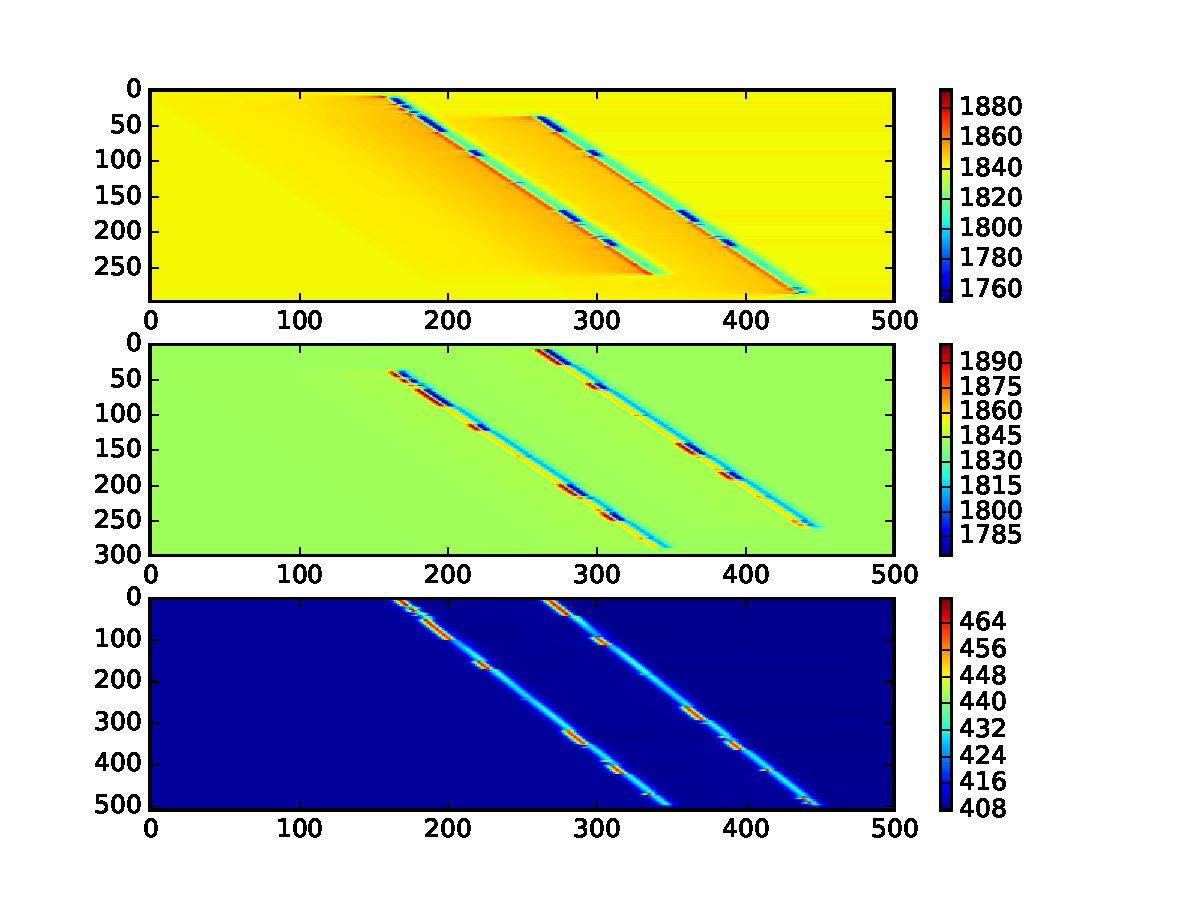
\includegraphics[height=0.6\textheight,clip,trim=15mm 1cm 0 1cm]{ideal-2tracks-uboone-uv-shorted-adc.pdf}

        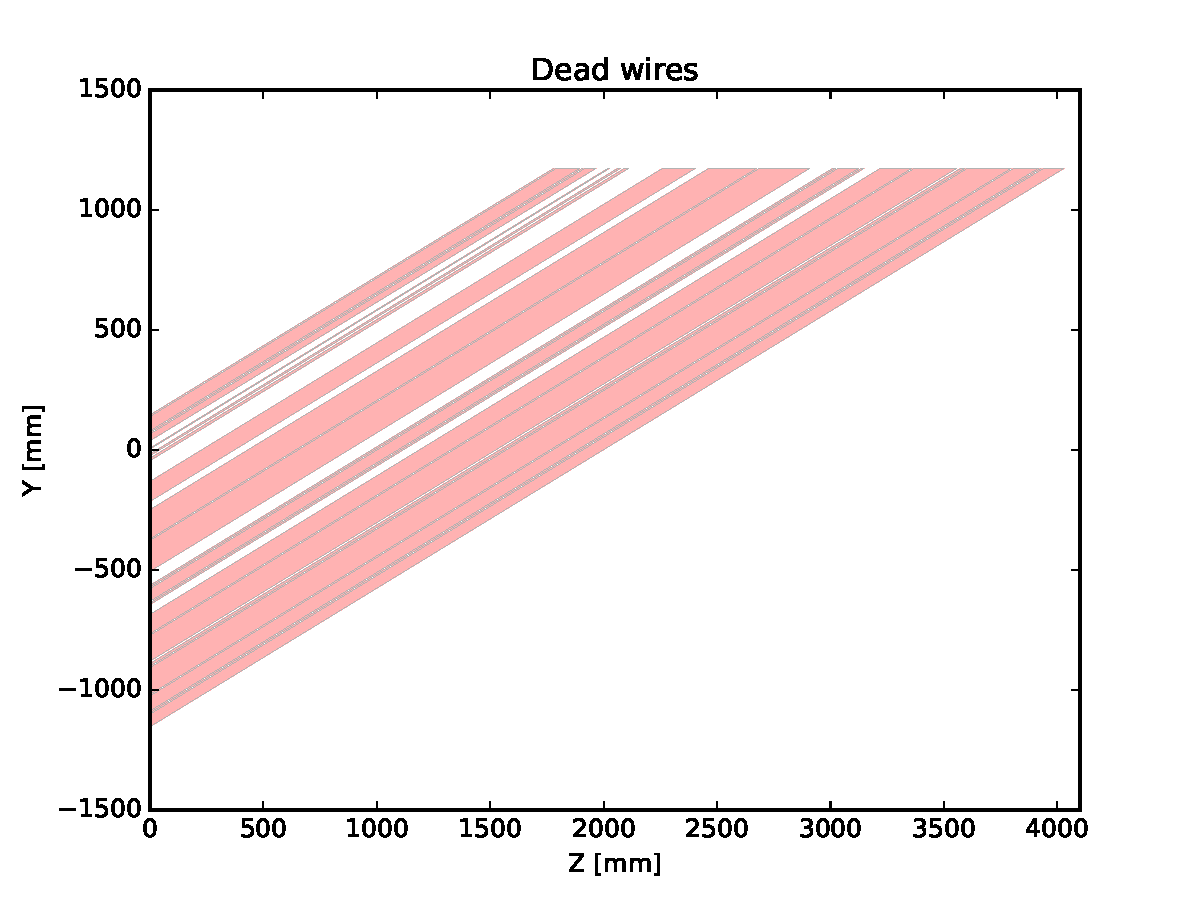
\includegraphics[height=0.3\textheight,page=1,clip,trim=0 0 0 13.7mm]{microboone-shorted-wires-v2.pdf}
      \end{center}
    \end{column}
    \begin{column}{0.5\textwidth}
      \begin{center}
        \scriptsize VY-grounded region

        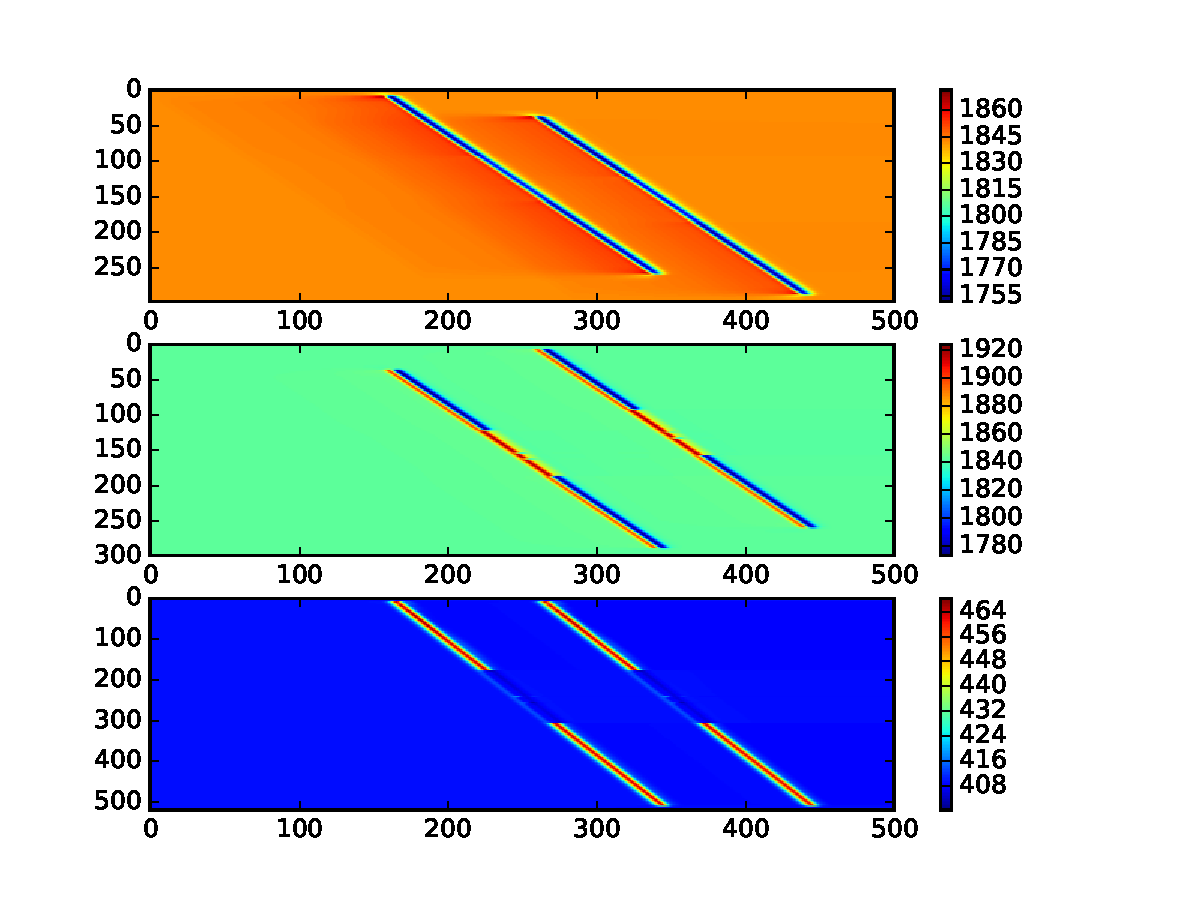
\includegraphics[height=0.6\textheight,clip,trim=15mm 1cm 0 1cm]{ideal-2tracks-uboone-vy-shorted-adc.pdf}

        \includegraphics[height=0.3\textheight,page=2,clip,trim=0 0 0 13.7mm]{microboone-shorted-wires-v2.pdf}
      \end{center}
    \end{column}
  \end{columns}

  \vspace{-20mm}

  \begin{center}
    \tiny (grounded wires)
  \end{center}
  

\end{frame}

\subsection{Noise}
\begin{frame}
  \tableofcontents[currentsection,hideothersubsections]
\end{frame}

\begin{frame}
  \frametitle{Simulated Noise}
  The fifth D: \textbf{dissonance}

  \begin{columns}
    \begin{column}{0.7\textwidth}
      \begin{itemize}\footnotesize
      \item Including the noise simulation in a job is a user-configurable optional.
      \item User-provided mean noise specta as function of wire length.
      \item Battery included: post-filtered spectra from MicroBooNE noise paper.
      \item Proper Rayleigh sampling when producing noise waveforms.
        \begin{itemize}\tiny
        \item[$\to$] todo: generating noise needs many randoms, which is
          rather slow. 
          Ideas on how to speed this up need implementation and validation.
        \end{itemize}
      \item[$\to$] todo: support for modeling coherent noise.
      \end{itemize}
    \end{column}
    \begin{column}{0.3\textwidth}

        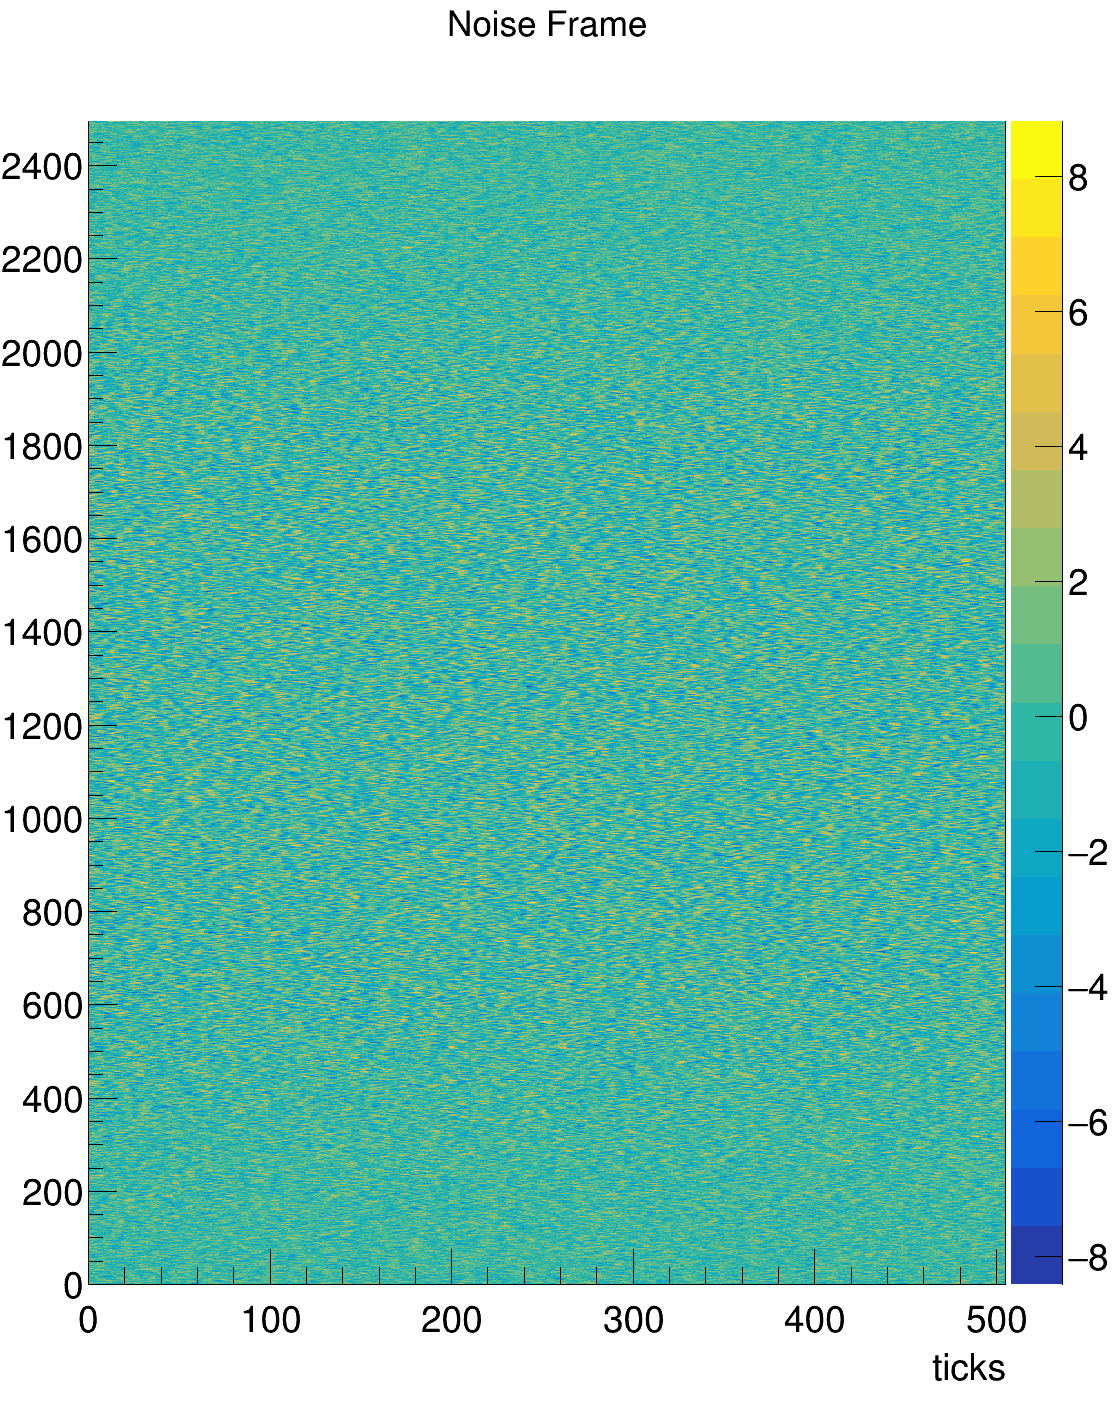
\includegraphics[width=\textwidth]{noise.png}

        \tiny
        Sampled noise spectra in channel vs tick for MB U-plane channels.

        Note variation as function of wire length.

    \end{column}
  \end{columns}

\end{frame}

\subsection{Mixing}
\begin{frame}
  \tableofcontents[currentsection,hideothersubsections]
\end{frame}

\begin{frame}
  \frametitle{Mixing}
  WCT simulation supports mixing at many levels.
  \begin{itemize}\footnotesize
  \item WCT inherently follows a \textbf{data flow processing} (DFP) paradigm.
    \begin{itemize}\scriptsize
    \item[o] constrast: \textit{art} follows an ``event'' (blocked) processing paradigm.
    \end{itemize}
  \item DFP naturally supports ``mixing'' of data streams.
    \begin{itemize}\scriptsize
    \item[o] Not just for sim, but any WCT job.
    \end{itemize}
  \item WCT simulation could mix multiple sources of:
    \begin{itemize}\scriptsize
    \item[o] depos, each one type of kinematics (cosmic, beam, $^{39}$Ar, dirt)
    \item[o] frames, noise+signal, \texttt{MultiDuctor}, data+sim
    \end{itemize}
  \end{itemize}

  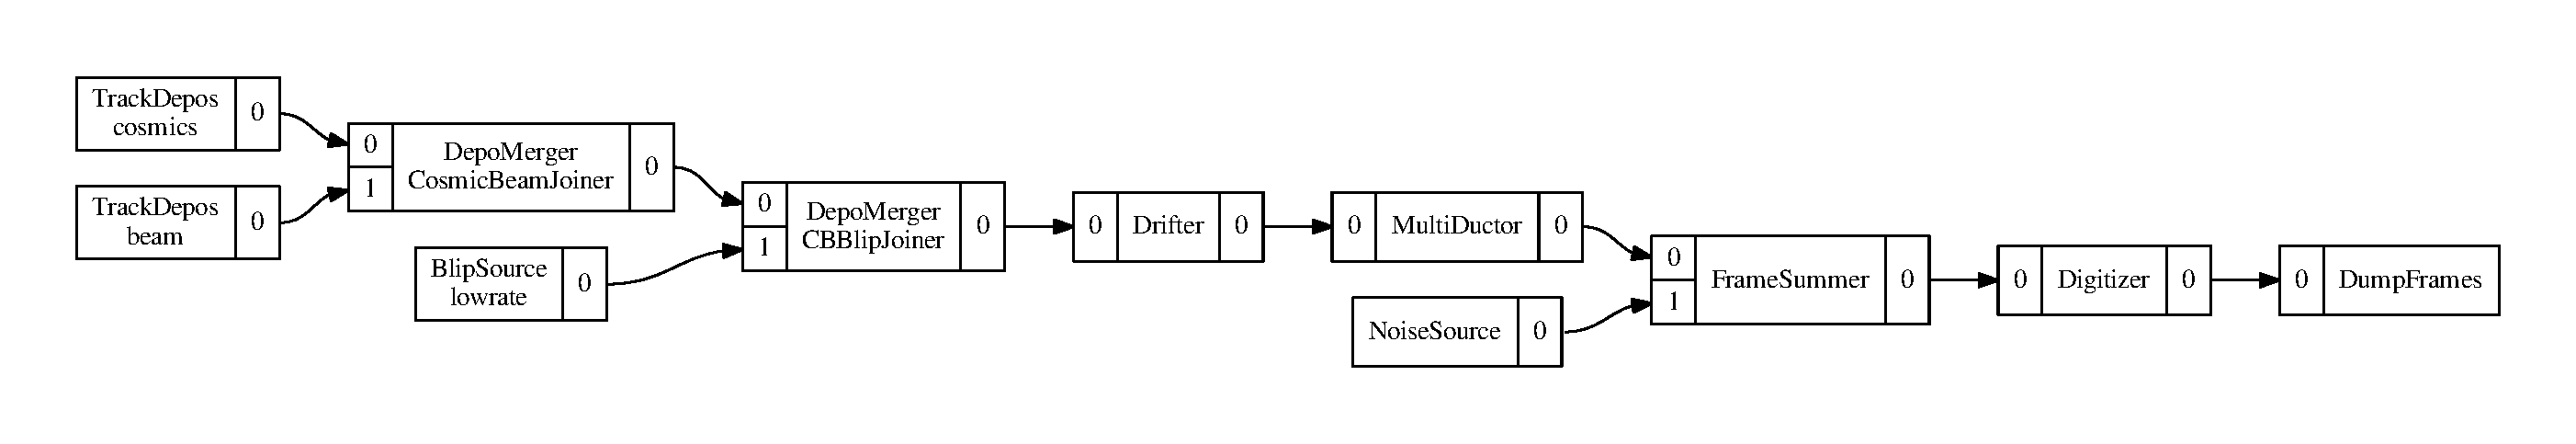
\includegraphics[width=\textwidth]{mixing.pdf}
\end{frame}

\subsection{DFP Graph}
\begin{frame}
  \frametitle{DFP Graph Execution}
  New support for DFP graph execution:
  \begin{itemize}\footnotesize
  \item Prior, most WCT ``app'' components hard-coded execution paths.
    \begin{itemize}\tiny
    \item If you squint at the C++ you might see a directed acyclic graph.
    \end{itemize}
  \item New: \texttt{Pgrapher}, a single-threaded, memory-minimizing
    DFP graph execution engine
  \item Can now construct many variants of a full WCT job simply in
    WCT configuration by effectively ``drawing'' the graph.
    \begin{itemize}\scriptsize
    \item[o] Eg, this graph is generated directly from a WCT configuration:
    \end{itemize}
  \end{itemize}
  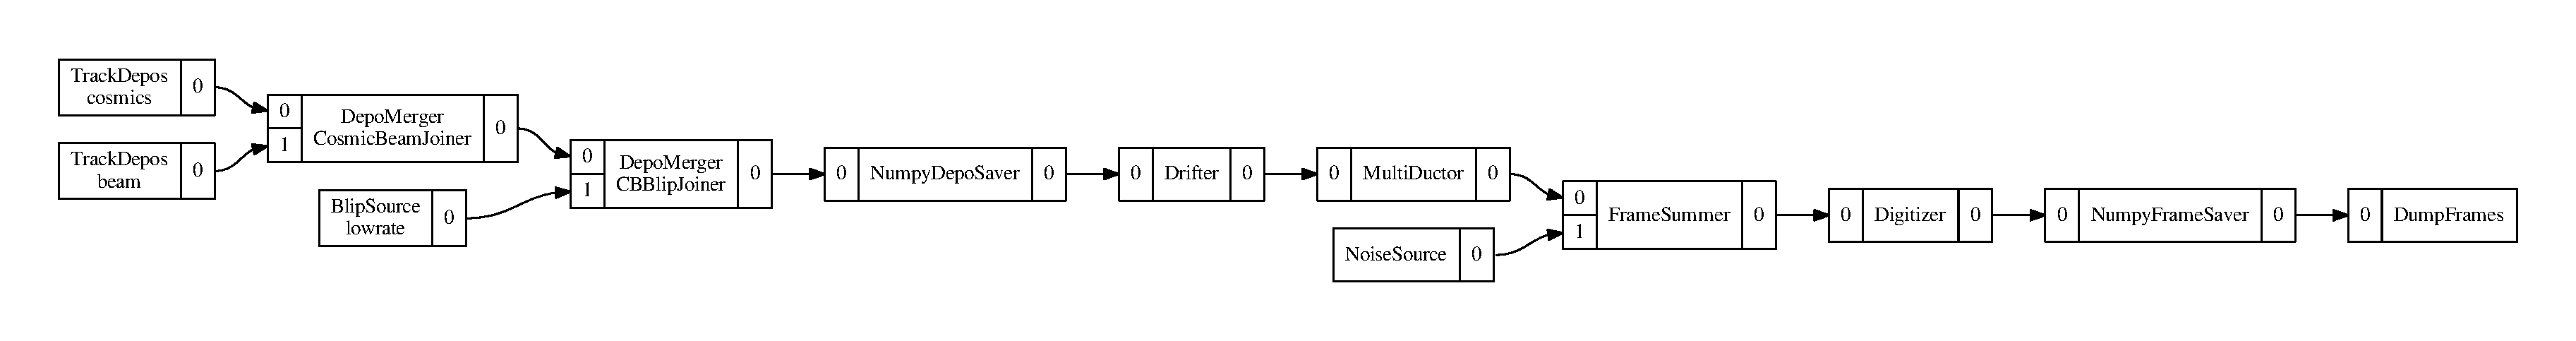
\includegraphics[width=\textwidth]{test_simgraph_noise.pdf}

  \tiny todo: a multi-threaded DFP graph execution engine also exists
  in WCT but needs validation. 
  It most likely can only reap benefit in stand-alone
  \texttt{wire-cell} on HPC (outside of a monolithic larsoft).

\end{frame}

\section{Integration of WCT sim to LArSoft}
\begin{frame}
  \tableofcontents[currentsection,hideothersubsections]
\end{frame}

\begin{frame}
  \frametitle{WC/LS Integration Design}

  \begin{itemize}\footnotesize
  \item WCT components that \textbf{convert} between WCT data
    interfaces and \texttt{art::Event} data objects.
  \item WCT components that \textbf{adapt} LS services.
  \item The (mostly empty) \texttt{WireCellToolkit\_module} which uses:
  \item The \texttt{WCLS\_tool}  which executes WCT ``apps''
    \begin{itemize}\scriptsize
    \item[o] This \texttt{art::Tool} is to \textit{art} what
      \texttt{wire-cell} is to your shell command line.
    \item[o] What might be on the command line is provided in FHiCL.
    \item[o] Largely identical WCT config works for WC/LS or stand-alone WCT running.
    \end{itemize}
  \end{itemize}

  \begin{center}
    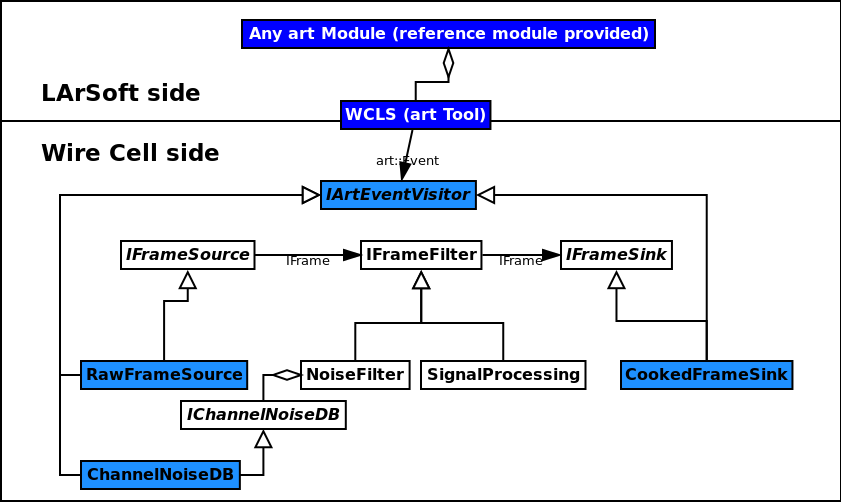
\includegraphics[height=3cm]{nfsp-integ.pdf}
  \end{center}

\end{frame}

\begin{frame}
  \frametitle{WC/LS Code \& Config}

  \begin{itemize}
  \item Integration code is in the \texttt{larwirecell} package, part
    of the base LArSoft family.
    \begin{itemize}\scriptsize
    \item[o] Development is against \texttt{master} not the ancient MB
      ``production'' branches.
    \item[o] Package only holds integration glue and essentially no
      ``real'' code except for some ``impedance matching'' modules.
    \end{itemize}
  \item Compiled WCT code is provided by the \texttt{wirecell} UPS
    product as an ``external'' package.
    \begin{itemize}\scriptsize
    \item[o] Subset of releases made in upstream WCT become UPS'ified.
    \end{itemize}
  \item WCT configuration files (including ``data'' files such as for
    field response, noise spectra) are provided by the user and found
    by WCT via the \texttt{WIRECELL\_PATH} env. var.
  \end{itemize}
\end{frame}

\begin{frame}
  \frametitle{WC/LS Status and Work Needed}
  \begin{itemize}\footnotesize
  \item Noise filter + signal processing is integrated and in use.
    \begin{itemize}\scriptsize
    \item[o] WCT config uses hard-wired \texttt{Omnibus} ``app'', may move to \texttt{Pgrapher}.
    \end{itemize}
  \item Simulation integration already ``done''
    \begin{itemize}\scriptsize
    \item[o] Full \texttt{art::Event} $\to$ WCT $\to$ \texttt{art::Event} for the ``4 D's'' for single ``event''.
      \begin{itemize}\tiny
      \item (took four hours of fighting \texttt{mrb} and 30 minutes of actual coding)
      \end{itemize}
    \item[o] Minor work on WCT needed to better adapt WCT's DFP to \textit{art}'s
      ``event'' based processing paradigms.
    \item[o] I have copied \texttt{SimEnergyDeposit} into my own
      recent branch of \texttt{lardataobj}.
      \begin{itemize}\tiny
      \item Will push to merge my \texttt{lardataobj} branch to \texttt{master}.
      \item For testing, I simply generate depos for a line source.
      \item Getting LArG4 or other sources to produce depos left as an exercise for the user.
      \end{itemize}
    \end{itemize}

  \end{itemize}
\end{frame}

\end{document}

